\chapter{Survey}
\label{chp:amtsurvey} 

\section{Constructing the Survey}

\subsection{How and why we chose this design}
%hvorfor vi satte spørsmålene der vi gjorde osv osv. Design!
%Hvorfor surveymonkey?
%hvordan vi gikk fram på AMT? hvorfor amt?

\section{Survey Results}
%Hvordan vi har gått gjennom resultatene, hva vi har fokusert på og hvorfor!

\subsection{Demographics}
Gender:
Male: 108 (43,20\%)
Female: 142 (56,80\%)
%and so on

\begin{figure}[h!]
\centering
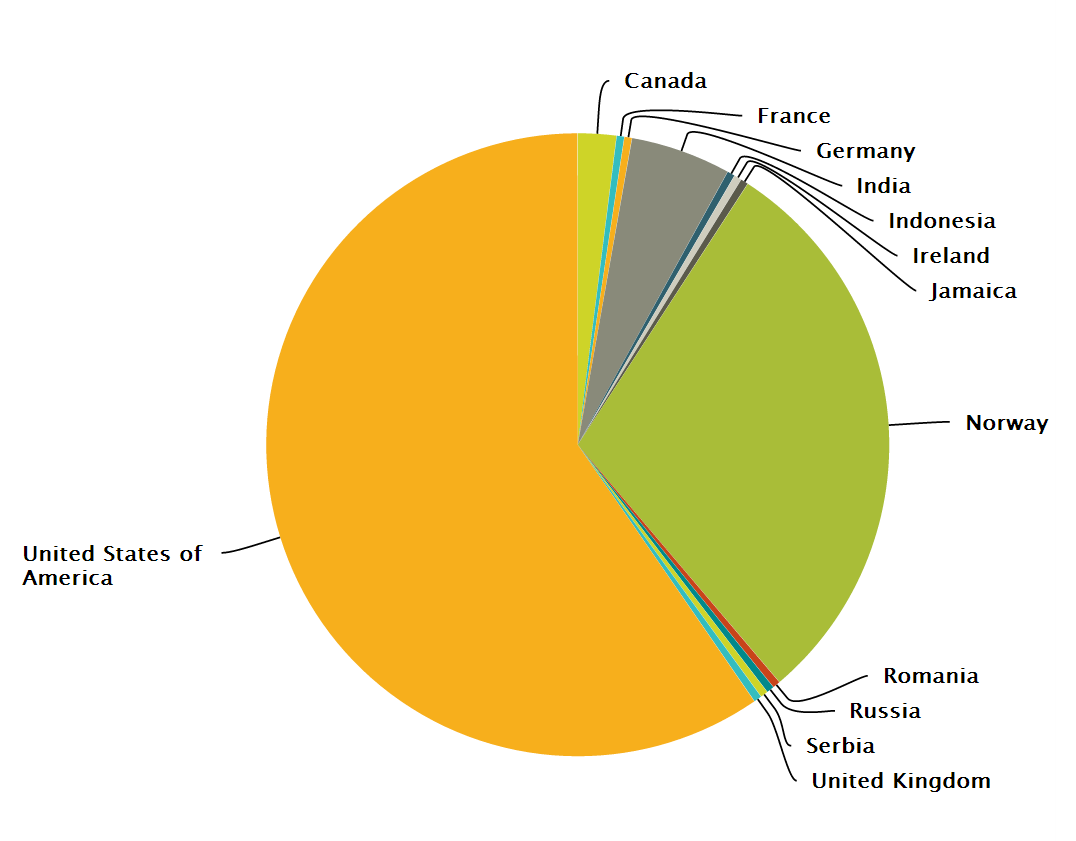
\includegraphics[width=1\textwidth]{land.png}
\caption[Bilde 1]{Bilde 11} 
\label{fig:co}
\end{figure}

\subsection{Never Checked Facebook Privacy Settings During the Last Year}
% De som svarte "never checked" på Q3
30 of the people who answered our survey stated that they have never checked their privacy settings during the last year. Even though they have not checked the privacy settings during the last year, most of them have done some changes to their settings before the previous year. 

Average number of friends: 162
Average age: 39

\begin{figure}[h!]
\centering
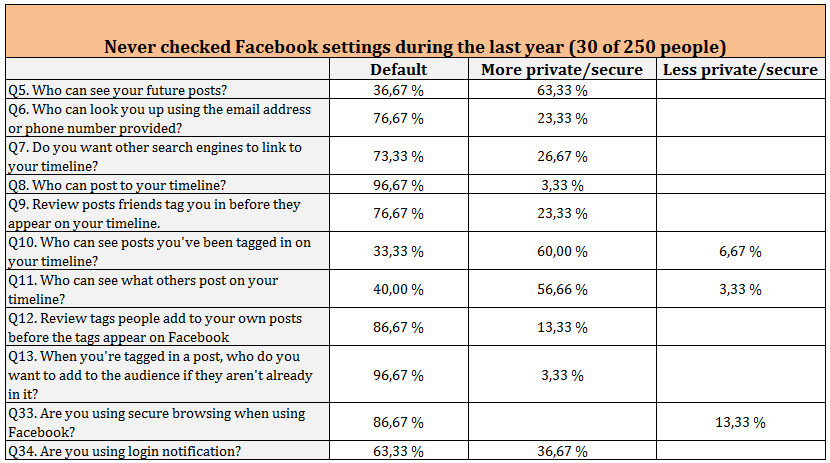
\includegraphics[width=1\textwidth]{nevercheckedtable.png}
\caption[Bilde 1]{Bilde 11} 
\label{fig:co}
\end{figure}

60\% did not consider changing privacy settings after reviewing them. 
40\% wanted to make their privacy settings more private. 

Quote from \#2 on Question 23: "Now you have scared me. I am alone and afraid" -Random Female with Ph.D, 5 friends and 67 years old. 

For example under "Who can see your future posts?" 11 people answered public and 19 persons answered friends.
- Default is public

On the setting "Who can look me up? Do you want other search engines to link to your timeline?" 22 has it on (this is default), and 8 has turned it off. 

7 of them has enabled the "Review posts friends tag you in before they appear on your timeline". 

\subsection{Checks Privacy Settings "Once a month" or "Once a week or more"}
Average number of friends: 416
Average age: 28,5

85\% of these people checks their Facebook at least once a day.
70,83 \% did not consider changing privacy settings after reviewing them. 
27,08 \% wanted to make their privacy settings more private.
2,08\% considered changing them to more public 

12 of the 48 people in this category answered yes on the question whether or not facebook had affected their personal life negativally. Half of these had situations with friends posting unwanted pictures (av forskjellige grunner) of them.

One guy: Two accounts; one under a pseudonym for friends only and on with strict settings for the rest of the world. "Privacy is important to me. It is meaningless not to give others the same courtesy" - Random guy with 420 friends that are 43 years old. 

\begin{figure}[h!]
\centering
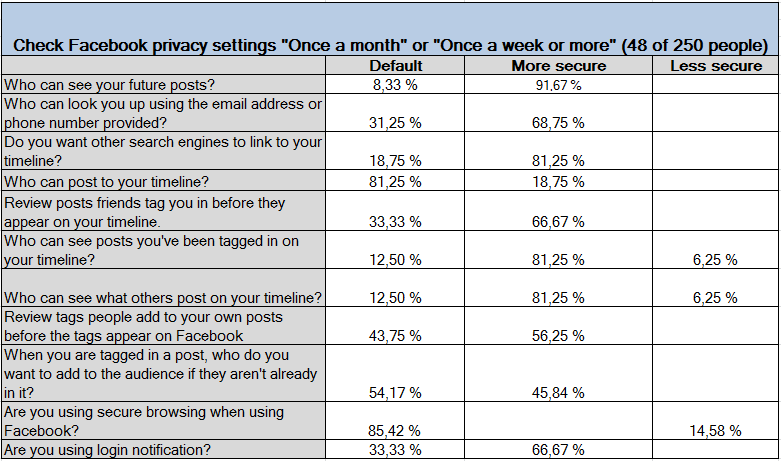
\includegraphics[width=1\textwidth]{checkonceaweekormoretable.png}
\caption[Bilde 1]{Bilde 11} 
\label{fig:co}
\end{figure}

\subsection{Interdependent Privacy}


